
% Kompilierung (�bersetzung): PdfLaTeX, BibTex, PdfLatex, Pdf-Anzeigeprogramm

\documentclass[xlevel, hyperref, mp, nat]{wise}

\newcommand{\bibtex}{\texorpdfstring{Bib\kern-.125em\TeX}{BibTeX}}

%Dokument beginnen
\begin{document}

%Das erste ist die Titelseite
%Bei lediglich einem Betreuer bitte den zweiten Betreuer samt Umbruchzeichen (\\) entfernen. 
%Wie Sie ihre Titelseite �ndern entnehmen Sie bitte der WiSe-Dokumentation. 
\seminartitlepage
{Seminararbeitstitel}
{Name des Studenten (Matrikelnummer) \\ Name des Studenten 2 (Matrikelnummer)}
{Titel und Name des Betreuers \\ Titel und Name des zweiten Betreuers}
{Studienfach}

%Vorpsann beginnen
\begin{preface}
  %Es folgt eine kurze Zusammenfassung der Arbeit
  \abstract
  

  %Inhaltsverzeichnis
  \tableofcontents
\end{preface}

%Mit der Einleitung beginnt der Hauptteil der Arbeit.
\introduction

Hier ist die Einleitung

%Dieser kann ganz normal mit \include{Dateiname} auch in
%mehrere Dateien zerlegt werden. Im Texmaker geben Sie dann ihre Arbeit.tex als Masterdatei an, damit Sie global eine �bersetzung f�r das gew�nschte Dokument starten k�nnen. Included Files werden dabei automatisch gespeichert. 

\section{Kapitel 1}
\label{sec:kapitel1}
% Diese Kapitel sind nur exemplarisch eingef�gt worden. Sie k�nnen die Namen zum Zweck ihrer Arbeit ver�ndern. 





\subsection{Abschnitt}
\label{sec:abschnitt}


\subsubsection{Unterabschnitt}
\label{sec:unterabschnitt}


\paragraph{Unterunterabschnitt}
\label{sec:unterunterabschnitt}

\subparagraph{Absatz}
\label{sec:absatz}

\section{Kapitel 2}
% Hier sehen Sie eine Beispielreferenz auf Kapitel 1:
Wie in Kapitel \ref{sec:kapitel1} erkl�rt wurde, gibt es das in Abb. \ref{abb:kette} dargestellte Flussdiagramm. Die Reihenfolge der erstellten Hilfsdateien und der Einbindung dieser in der n�chsten �bersetzung ist der Grund, warum eine bestimmte Kompilierungsreihenfolge (�bersetzungsreihenfolge) voreingestellt werden muss. Zuvor verwendete Verweise befinden sich in der bbl-Datei und es kann einfach mit pdflatex-viewpdf kompiliert werden. 

\begin{figure}[H]
\centering 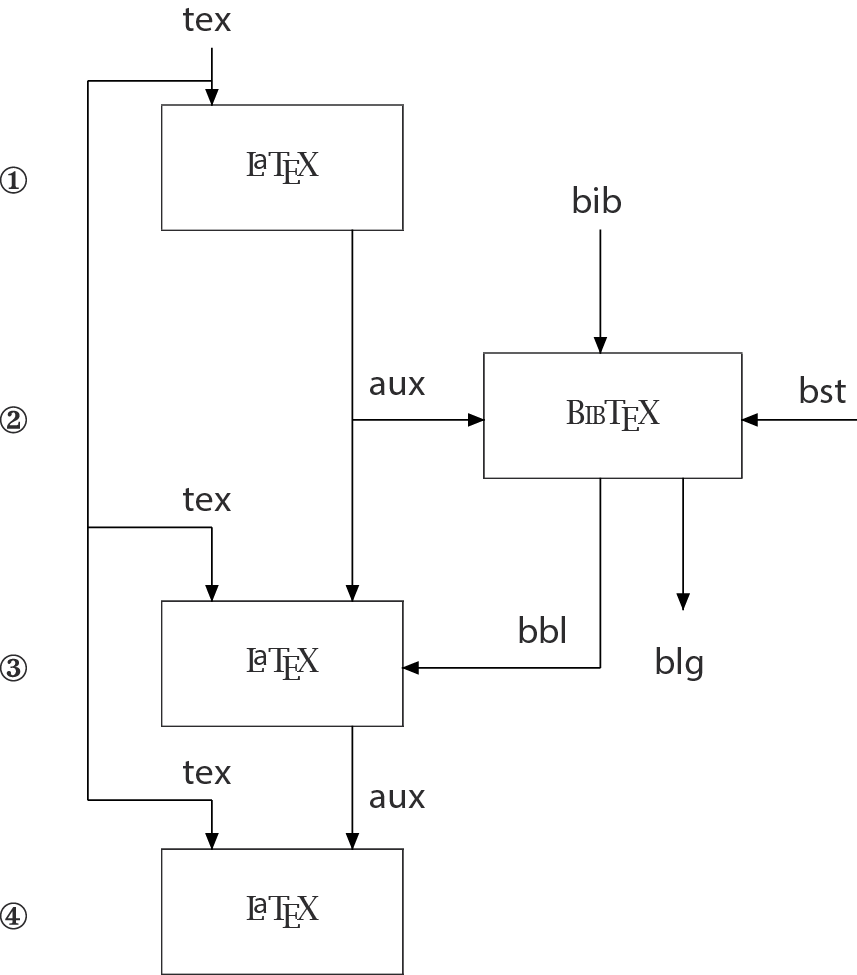
\includegraphics[width=\textwidth]{bilder/flussdiagramm01} 
\caption[Flu�diagramm des Zusammenspiels von \bibtex und \LaTeX]
{Flussdiagramm des Zusammenspiels von \bibtex und \LaTeX . Grafik entnommen aus (\cite{mittelbach05}. }
\label{abb:kette}
\end{figure}
% Der Eintrag  in eckigen Klammern ist der Text f�r den Verweis im Abbildungsverzeichnis, in geschweiften Klammern befindet sich die Bildunterschrift.  Die f�r das Abbildungsverzeichnis sollte k�rzer sein! 







%Die Arbeit schlie�t mit dem Anhang
\begin{appendix}  
  %Abbildungsverzeichnis
  \listoffigures

  %Tabellenverzeichnis
  \listoftables

  %Liste aller Abk�rzungen
  \listofabbreviations
  \abbreviation{bzw.}{beziehungsweise}
  \abbreviation{u.a.}{unter andrem}

  %Literaturverzeichnis unter Angabe der Literaturdatenbank
  %literatur.bib sollte von einem Literaturverwaltungsprogramm ge�ffnet und editiert werden. 
  \bibliography{literatur}
  \bibliographystyle{wisenat}
  \begin{appendices}
  %Anhang definieren
  \section{Das Megamodell der Systementwicklung}
  \newpage
  Hier geht das Megamodell weiter
  \subsection{Die Megasicht auf das Megamodell der Systementwicklung}

  \end{appendices}
  %Die Arbeit schlie�t mit der ehrenw�rtlichen Erkl�rung
  \declaration
\end{appendix}

\end{document}
